\chapter{Cây phân đoạn nâng cao}

\index{segment tree}

Cây phân đoạn là một cấu trúc dữ liệu đa năng
có thể được sử dụng để giải quyết một số lượng lớn các bài toán thuật toán.
Tuy nhiên, có nhiều chủ đề liên quan đến cây phân đoạn
mà chúng ta chưa đề cập đến.
Bây giờ là lúc để thảo luận về một số biến thể nâng cao hơn
của cây phân đoạn.

Cho đến nay, chúng ta đã triển khai các thao tác
của một cây phân đoạn bằng cách đi \emph{từ dưới lên trên}
trong cây.
Ví dụ, chúng ta đã tính
tổng phạm vi như sau (Chương 9.3):

\begin{lstlisting}
int sum(int a, int b) {
    a += n; b += n;
    int s = 0;
    while (a <= b) {
        if (a%2 == 1) s += tree[a++];
        if (b%2 == 0) s += tree[b--];
        a /= 2; b /= 2;
    }
    return s;
}
\end{lstlisting}

Tuy nhiên, trong các cây phân đoạn nâng cao hơn,
thường cần phải triển khai các thao tác
theo một cách khác, \emph{từ trên xuống dưới}.
Sử dụng cách tiếp cận này, hàm trở thành như sau:
\begin{lstlisting}
int sum(int a, int b, int k, int x, int y) {
    if (b < x || a > y) return 0;
    if (a <= x && y <= b) return tree[k];
    int d = (x+y)/2;
    return sum(a,b,2*k,x,d) + sum(a,b,2*k+1,d+1,y);
}
\end{lstlisting}

Bây giờ chúng ta có thể tính bất kỳ giá trị nào của $\texttt{sum}_q(a,b)$
(tổng các giá trị mảng trong phạm vi $[a,b]$) như sau:
\begin{lstlisting}
int s = sum(a, b, 1, 0, n-1);
\end{lstlisting}

Tham số $k$ chỉ ra vị trí hiện tại
trong \texttt{tree}.
Ban đầu $k$ bằng 1, bởi vì chúng ta bắt đầu
tại gốc của cây.
Phạm vi $[x,y]$ tương ứng với $k$
và ban đầu là $[0,n-1]$.
Khi tính tổng,
nếu $[x,y]$ nằm ngoài $[a,b]$,
tổng là 0,
và nếu $[x,y]$ hoàn toàn nằm trong $[a,b]$,
tổng có thể được tìm thấy trong \texttt{tree}.
Nếu $[x,y]$ một phần nằm trong $[a,b]$,
việc tìm kiếm tiếp tục một cách đệ quy đến
nửa trái và nửa phải của $[x,y]$.
Nửa trái là $[x,d]$
và nửa phải là $[d+1,y]$
trong đó $d=\lfloor \frac{x+y}{2} \rfloor$.

Hình sau cho thấy quá trình tìm kiếm diễn ra
khi tính giá trị của $\texttt{sum}_q(a,b)$.
Các nút màu xám chỉ ra các nút nơi đệ quy
dừng lại và tổng có thể được tìm thấy trong \texttt{tree}.

\begin{center}
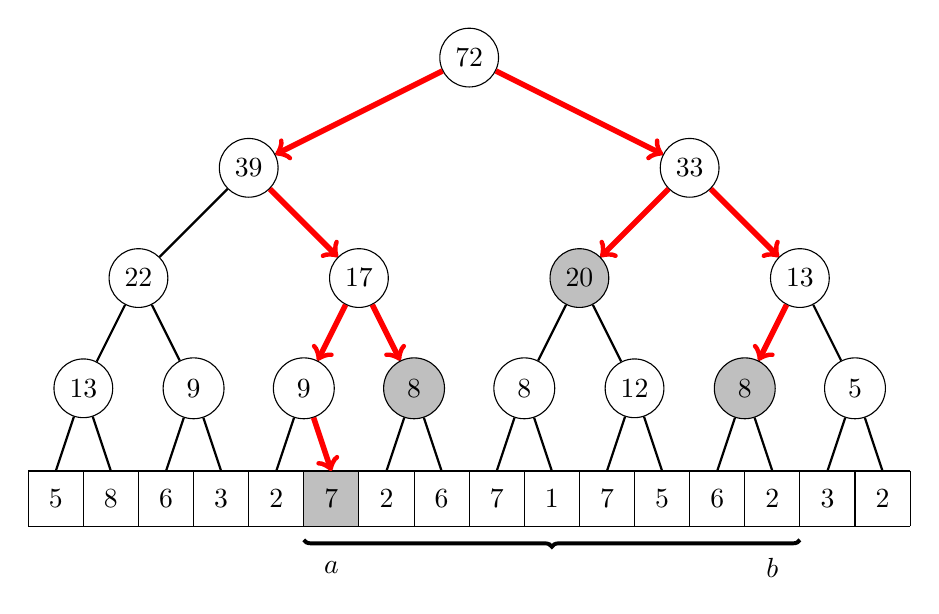
\begin{tikzpicture}[scale=0.7]
\fill[color=gray!50] (5,0) rectangle (6,1);
\draw (0,0) grid (16,1);

\node[anchor=center] at (0.5, 0.5) {5};
\node[anchor=center] at (1.5, 0.5) {8};
\node[anchor=center] at (2.5, 0.5) {6};
\node[anchor=center] at (3.5, 0.5) {3};
\node[anchor=center] at (4.5, 0.5) {2};
\node[anchor=center] at (5.5, 0.5) {7};
\node[anchor=center] at (6.5, 0.5) {2};
\node[anchor=center] at (7.5, 0.5) {6};
\node[anchor=center] at (8.5, 0.5) {7};
\node[anchor=center] at (9.5, 0.5) {1};
\node[anchor=center] at (10.5, 0.5) {7};
\node[anchor=center] at (11.5, 0.5) {5};
\node[anchor=center] at (12.5, 0.5) {6};
\node[anchor=center] at (13.5, 0.5) {2};
\node[anchor=center] at (14.5, 0.5) {3};
\node[anchor=center] at (15.5, 0.5) {2};

\node[draw, circle] (a) at (1,2.5) {13};
\path[draw,thick,-] (a) -- (0.5,1);
\path[draw,thick,-] (a) -- (1.5,1);
\node[draw, circle,minimum size=22pt] (b) at (3,2.5) {9};
\path[draw,thick,-] (b) -- (2.5,1);
\path[draw,thick,-] (b) -- (3.5,1);
\node[draw, circle,minimum size=22pt] (c) at (5,2.5) {9};
\path[draw,thick,-] (c) -- (4.5,1);
\path[draw,thick,-] (c) -- (5.5,1);
\node[draw, circle,fill=gray!50,minimum size=22pt] (d) at (7,2.5) {8};
\path[draw,thick,-] (d) -- (6.5,1);
\path[draw,thick,-] (d) -- (7.5,1);
\node[draw, circle,minimum size=22pt] (e) at (9,2.5) {8};
\path[draw,thick,-] (e) -- (8.5,1);
\path[draw,thick,-] (e) -- (9.5,1);
\node[draw, circle] (f) at (11,2.5) {12};
\path[draw,thick,-] (f) -- (10.5,1);
\path[draw,thick,-] (f) -- (11.5,1);
\node[draw, circle,fill=gray!50,minimum size=22pt] (g) at (13,2.5) {8};
\path[draw,thick,-] (g) -- (12.5,1);
\path[draw,thick,-] (g) -- (13.5,1);
\node[draw, circle,minimum size=22pt] (h) at (15,2.5) {5};
\path[draw,thick,-] (h) -- (14.5,1);
\path[draw,thick,-] (h) -- (15.5,1);

\node[draw, circle] (i) at (2,4.5) {22};
\path[draw,thick,-] (i) -- (a);
\path[draw,thick,-] (i) -- (b);
\node[draw, circle] (j) at (6,4.5) {17};
\path[draw,thick,-] (j) -- (c);
\path[draw,thick,-] (j) -- (d);
\node[draw, circle,fill=gray!50] (k) at (10,4.5) {20};
\path[draw,thick,-] (k) -- (e);
\path[draw,thick,-] (k) -- (f);
\node[draw, circle] (l) at (14,4.5) {13};
\path[draw,thick,-] (l) -- (g);
\path[draw,thick,-] (l) -- (h);

\node[draw, circle] (m) at (4,6.5) {39};
\path[draw,thick,-] (m) -- (i);
\path[draw,thick,-] (m) -- (j);
\node[draw, circle] (n) at (12,6.5) {33};
\path[draw,thick,-] (n) -- (k);
\path[draw,thick,-] (n) -- (l);

\node[draw, circle] (o) at (8,8.5) {72};
\path[draw,thick,-] (o) -- (m);
\path[draw,thick,-] (o) -- (n);

\path[draw=red,thick,->,line width=2pt] (o) -- (m);
\path[draw=red,thick,->,line width=2pt] (o) -- (n);

\path[draw=red,thick,->,line width=2pt] (m) -- (j);
\path[draw=red,thick,->,line width=2pt] (j) -- (c);
\path[draw=red,thick,->,line width=2pt] (j) -- (d);
\path[draw=red,thick,->,line width=2pt] (c) -- (5.5,1);

\path[draw=red,thick,->,line width=2pt] (n) -- (k);
\path[draw=red,thick,->,line width=2pt] (n) -- (l);

\path[draw=red,thick,->,line width=2pt] (l) -- (g);

\draw [decoration={brace}, decorate, line width=0.5mm] (14,-0.25) -- (5,-0.25);

\node at (5.5,-0.75) {$a$};
\node at (13.5,-0.75) {$b$};
\end{tikzpicture}
\end{center}

Cũng trong cách triển khai này,
các thao tác mất thời gian $O(\log n)$,
bởi vì tổng số nút được duyệt là $O(\log n)$.

\section{Truyền lười (Lazy propagation)}

\index{lazy propagation}
\index{lazy segment tree}

Sử dụng \key{truyền lười (lazy propagation)}, chúng ta có thể xây dựng
một cây phân đoạn hỗ trợ \emph{cả} cập nhật phạm vi
và truy vấn phạm vi trong thời gian $O(\log n)$.
Ý tưởng là thực hiện các cập nhật và truy vấn
từ trên xuống dưới và thực hiện các cập nhật
một cách \emph{lười biếng} để chúng được truyền
xuống cây chỉ khi cần thiết.

Trong một cây phân đoạn lười biếng, các nút chứa hai loại
thông tin.
Giống như trong một cây phân đoạn thông thường,
mỗi nút chứa tổng hoặc một giá trị khác
liên quan đến mảng con tương ứng.
Ngoài ra, nút có thể chứa thông tin
liên quan đến các cập nhật lười biếng, chưa được
truyền đến các con của nó.

Có hai loại cập nhật phạm vi:
mỗi giá trị mảng trong phạm vi hoặc là
được \emph{tăng} lên một giá trị nào đó
hoặc được \emph{gán} một giá trị nào đó.
Cả hai thao tác có thể được triển khai bằng cách sử dụng
các ý tưởng tương tự, và thậm chí có thể xây dựng
một cây hỗ trợ cả hai thao tác cùng một lúc.

\subsubsection{Cây phân đoạn lười biếng}

Hãy xem xét một ví dụ trong đó mục tiêu của chúng ta là
xây dựng một cây phân đoạn hỗ trợ
hai thao tác: tăng mỗi giá trị trong
$[a,b]$ lên một hằng số và tính tổng các
giá trị trong $[a,b]$.

Chúng ta sẽ xây dựng một cây trong đó mỗi nút
có hai giá trị $s/z$:
$s$ biểu thị tổng các giá trị trong phạm vi,
và $z$ biểu thị giá trị của một cập nhật lười biếng,
có nghĩa là tất cả các giá trị trong phạm vi
nên được tăng lên $z$.
Trong cây sau, $z=0$ ở tất cả các nút,
vì vậy không có cập nhật lười biếng nào đang diễn ra.
\begin{center}
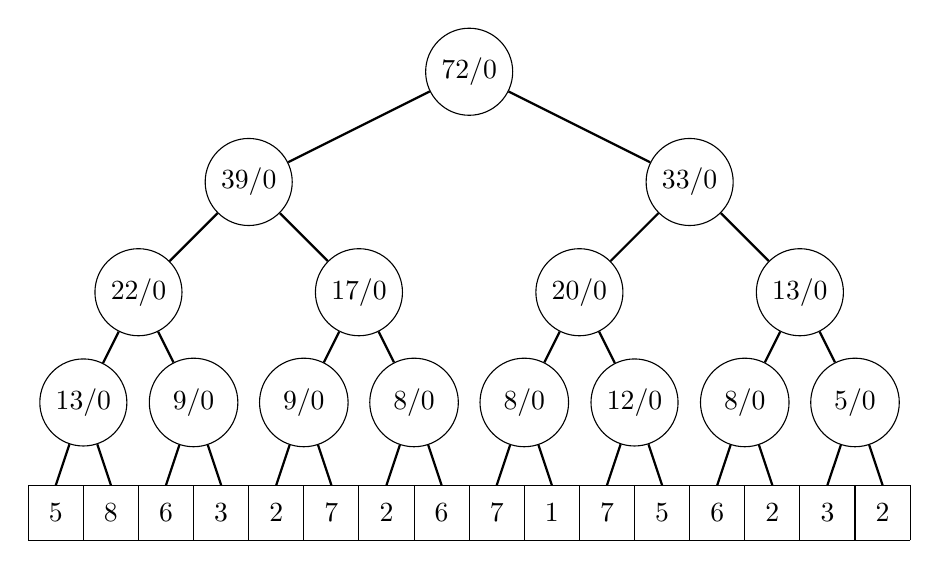
\begin{tikzpicture}[scale=0.7]
\draw (0,0) grid (16,1);

\node[anchor=center] at (0.5, 0.5) {5};
\node[anchor=center] at (1.5, 0.5) {8};
\node[anchor=center] at (2.5, 0.5) {6};
\node[anchor=center] at (3.5, 0.5) {3};
\node[anchor=center] at (4.5, 0.5) {2};
\node[anchor=center] at (5.5, 0.5) {7};
\node[anchor=center] at (6.5, 0.5) {2};
\node[anchor=center] at (7.5, 0.5) {6};
\node[anchor=center] at (8.5, 0.5) {7};
\node[anchor=center] at (9.5, 0.5) {1};
\node[anchor=center] at (10.5, 0.5) {7};
\node[anchor=center] at (11.5, 0.5) {5};
\node[anchor=center] at (12.5, 0.5) {6};
\node[anchor=center] at (13.5, 0.5) {2};
\node[anchor=center] at (14.5, 0.5) {3};
\node[anchor=center] at (15.5, 0.5) {2};

\node[draw, circle] (a) at (1,2.5) {13/0};
\path[draw,thick,-] (a) -- (0.5,1);
\path[draw,thick,-] (a) -- (1.5,1);
\node[draw, circle,minimum size=32pt] (b) at (3,2.5) {9/0};
\path[draw,thick,-] (b) -- (2.5,1);
\path[draw,thick,-] (b) -- (3.5,1);
\node[draw, circle,minimum size=32pt] (c) at (5,2.5) {9/0};
\path[draw,thick,-] (c) -- (4.5,1);
\path[draw,thick,-] (c) -- (5.5,1);
\node[draw, circle,minimum size=32pt] (d) at (7,2.5) {8/0};
\path[draw,thick,-] (d) -- (6.5,1);
\path[draw,thick,-] (d) -- (7.5,1);
\node[draw, circle,minimum size=32pt] (e) at (9,2.5) {8/0};
\path[draw,thick,-] (e) -- (8.5,1);
\path[draw,thick,-] (e) -- (9.5,1);
\node[draw, circle] (f) at (11,2.5) {12/0};
\path[draw,thick,-] (f) -- (10.5,1);
\path[draw,thick,-] (f) -- (11.5,1);
\node[draw, circle,minimum size=32pt] (g) at (13,2.5) {8/0};
\path[draw,thick,-] (g) -- (12.5,1);
\path[draw,thick,-] (g) -- (13.5,1);
\node[draw, circle,minimum size=32pt] (h) at (15,2.5) {5/0};
\path[draw,thick,-] (h) -- (14.5,1);
\path[draw,thick,-] (h) -- (15.5,1);

\node[draw, circle] (i) at (2,4.5) {22/0};
\path[draw,thick,-] (i) -- (a);
\path[draw,thick,-] (i) -- (b);
\node[draw, circle] (j) at (6,4.5) {17/0};
\path[draw,thick,-] (j) -- (c);
\path[draw,thick,-] (j) -- (d);
\node[draw, circle] (k) at (10,4.5) {20/0};
\path[draw,thick,-] (k) -- (e);
\path[draw,thick,-] (k) -- (f);
\node[draw, circle] (l) at (14,4.5) {13/0};
\path[draw,thick,-] (l) -- (g);
\path[draw,thick,-] (l) -- (h);

\node[draw, circle] (m) at (4,6.5) {39/0};
\path[draw,thick,-] (m) -- (i);
\path[draw,thick,-] (m) -- (j);
\node[draw, circle] (n) at (12,6.5) {33/0};
\path[draw,thick,-] (n) -- (k);
\path[draw,thick,-] (n) -- (l);

\node[draw, circle] (o) at (8,8.5) {72/0};
\path[draw,thick,-] (o) -- (m);
\path[draw,thick,-] (o) -- (n);
\end{tikzpicture}
\end{center}

Khi các phần tử trong $[a,b]$ được tăng lên $u$,
chúng ta đi từ gốc đến các lá
và sửa đổi các nút của cây như sau:
Nếu phạm vi $[x,y]$ của một nút
hoàn toàn nằm trong $[a,b]$,
chúng ta tăng giá trị $z$ của nút lên $u$ và dừng lại.
Nếu $[x,y]$ chỉ một phần thuộc về $[a,b]$,
chúng ta tăng giá trị $s$ của nút lên $hu$,
trong đó $h$ là kích thước của giao của $[a,b]$
và $[x,y]$, và tiếp tục đi một cách đệ quy trong cây.

Ví dụ, hình sau cho thấy cây sau khi
tăng các phần tử trong $[a,b]$ lên 2:
\begin{center}
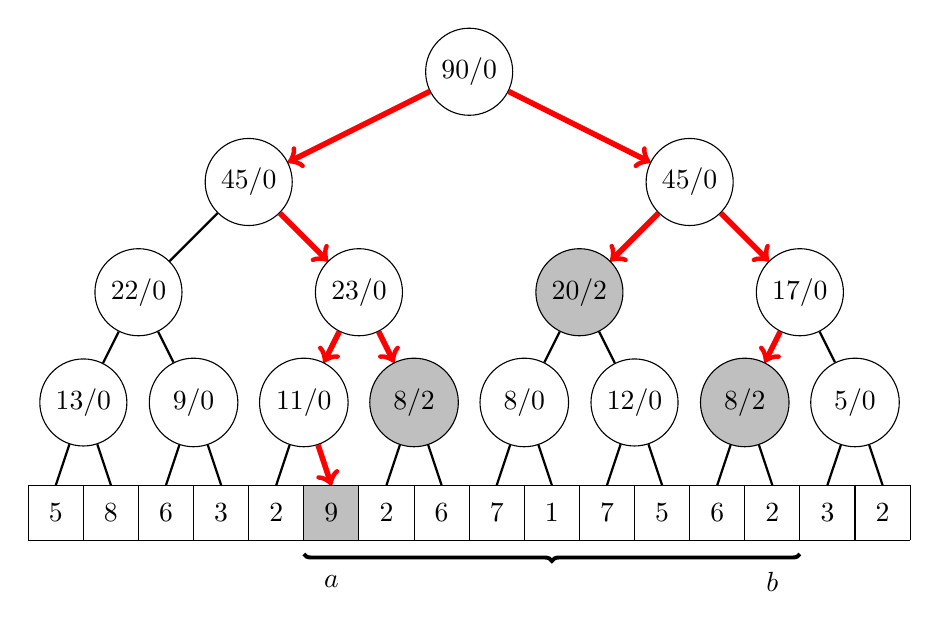
\begin{tikzpicture}[scale=0.7]
\fill[color=gray!50] (5,0) rectangle (6,1);
\draw (0,0) grid (16,1);

\node[anchor=center] at (0.5, 0.5) {5};
\node[anchor=center] at (1.5, 0.5) {8};
\node[anchor=center] at (2.5, 0.5) {6};
\node[anchor=center] at (3.5, 0.5) {3};
\node[anchor=center] at (4.5, 0.5) {2};
\node[anchor=center] at (5.5, 0.5) {9};
\node[anchor=center] at (6.5, 0.5) {2};
\node[anchor=center] at (7.5, 0.5) {6};
\node[anchor=center] at (8.5, 0.5) {7};
\node[anchor=center] at (9.5, 0.5) {1};
\node[anchor=center] at (10.5, 0.5) {7};
\node[anchor=center] at (11.5, 0.5) {5};
\node[anchor=center] at (12.5, 0.5) {6};
\node[anchor=center] at (13.5, 0.5) {2};
\node[anchor=center] at (14.5, 0.5) {3};
\node[anchor=center] at (15.5, 0.5) {2};

\node[draw, circle] (a) at (1,2.5) {13/0};
\path[draw,thick,-] (a) -- (0.5,1);
\path[draw,thick,-] (a) -- (1.5,1);
\node[draw, circle,minimum size=32pt] (b) at (3,2.5) {9/0};
\path[draw,thick,-] (b) -- (2.5,1);
\path[draw,thick,-] (b) -- (3.5,1);
\node[draw, circle,minimum size=32pt] (c) at (5,2.5) {11/0};
\path[draw,thick,-] (c) -- (4.5,1);
\path[draw,thick,-] (c) -- (5.5,1);
\node[draw, circle,fill=gray!50,minimum size=32pt] (d) at (7,2.5) {8/2};
\path[draw,thick,-] (d) -- (6.5,1);
\path[draw,thick,-] (d) -- (7.5,1);
\node[draw, circle,minimum size=32pt] (e) at (9,2.5) {8/0};
\path[draw,thick,-] (e) -- (8.5,1);
\path[draw,thick,-] (e) -- (9.5,1);
\node[draw, circle] (f) at (11,2.5) {12/0};
\path[draw,thick,-] (f) -- (10.5,1);
\path[draw,thick,-] (f) -- (11.5,1);
\node[draw, circle,fill=gray!50,minimum size=32pt] (g) at (13,2.5) {8/2};
\path[draw,thick,-] (g) -- (12.5,1);
\path[draw,thick,-] (g) -- (13.5,1);
\node[draw, circle,minimum size=32pt] (h) at (15,2.5) {5/0};
\path[draw,thick,-] (h) -- (14.5,1);
\path[draw,thick,-] (h) -- (15.5,1);

\node[draw, circle] (i) at (2,4.5) {22/0};
\path[draw,thick,-] (i) -- (a);
\path[draw,thick,-] (i) -- (b);
\node[draw, circle] (j) at (6,4.5) {23/0};
\path[draw,thick,-] (j) -- (c);
\path[draw,thick,-] (j) -- (d);
\node[draw, circle,fill=gray!50] (k) at (10,4.5) {20/2};
\path[draw,thick,-] (k) -- (e);
\path[draw,thick,-] (k) -- (f);
\node[draw, circle] (l) at (14,4.5) {17/0};
\path[draw,thick,-] (l) -- (g);
\path[draw,thick,-] (l) -- (h);

\node[draw, circle] (m) at (4,6.5) {45/0};
\path[draw,thick,-] (m) -- (i);
\path[draw,thick,-] (m) -- (j);
\node[draw, circle] (n) at (12,6.5) {45/0};
\path[draw,thick,-] (n) -- (k);
\path[draw,thick,-] (n) -- (l);

\node[draw, circle] (o) at (8,8.5) {90/0};
\path[draw,thick,-] (o) -- (m);
\path[draw,thick,-] (o) -- (n);

\path[draw=red,thick,->,line width=2pt] (o) -- (m);
\path[draw=red,thick,->,line width=2pt] (o) -- (n);

\path[draw=red,thick,->,line width=2pt] (m) -- (j);
\path[draw=red,thick,->,line width=2pt] (j) -- (c);
\path[draw=red,thick,->,line width=2pt] (j) -- (d);
\path[draw=red,thick,->,line width=2pt] (c) -- (5.5,1);

\path[draw=red,thick,->,line width=2pt] (n) -- (k);
\path[draw=red,thick,->,line width=2pt] (n) -- (l);

\path[draw=red,thick,->,line width=2pt] (l) -- (g);

\draw [decoration={brace}, decorate, line width=0.5mm] (14,-0.25) -- (5,-0.25);

\node at (5.5,-0.75) {$a$};
\node at (13.5,-0.75) {$b$};
\end{tikzpicture}
\end{center}

Chúng ta cũng tính tổng các phần tử trong một phạm vi $[a,b]$
bằng cách đi trong cây từ trên xuống dưới.
Nếu phạm vi $[x,y]$ của một nút hoàn toàn thuộc về
$[a,b]$, chúng ta cộng giá trị $s$ của nút đó vào tổng.
Ngược lại, chúng ta tiếp tục tìm kiếm một cách đệ quy
xuống dưới trong cây.

Cả trong cập nhật và truy vấn,
giá trị của một cập nhật lười biếng luôn được truyền
đến các con của nút
trước khi xử lý nút.
Ý tưởng là các cập nhật sẽ được truyền
xuống dưới chỉ khi cần thiết,
điều này đảm bảo rằng các thao tác luôn hiệu quả.

Hình sau cho thấy cây thay đổi như thế nào
khi chúng ta tính giá trị của $\texttt{sum}_a(a,b)$.
Hình chữ nhật cho thấy các nút có giá trị thay đổi,
bởi vì một cập nhật lười biếng được truyền xuống dưới.

\begin{center}
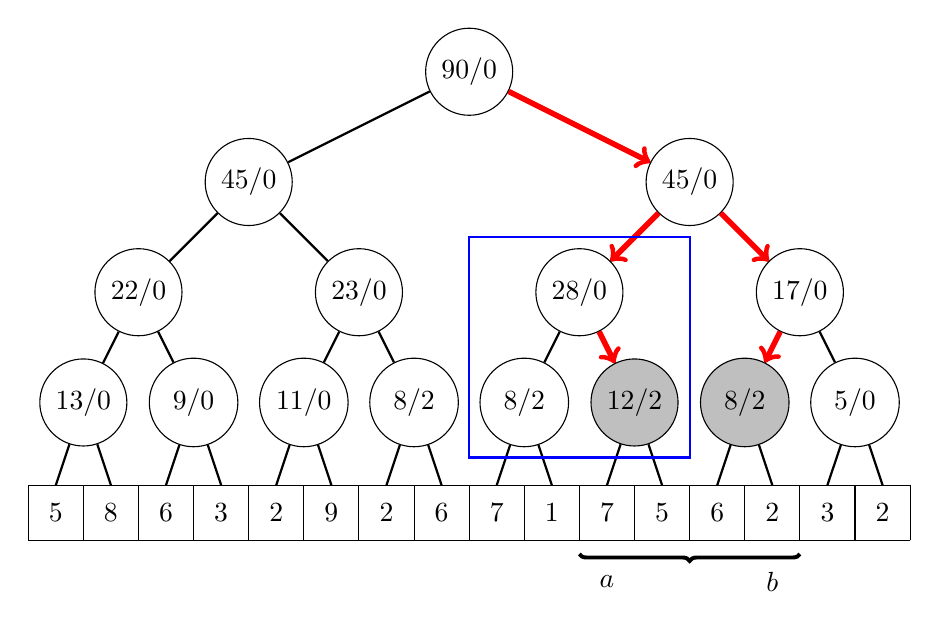
\begin{tikzpicture}[scale=0.7]
\draw (0,0) grid (16,1);

\node[anchor=center] at (0.5, 0.5) {5};
\node[anchor=center] at (1.5, 0.5) {8};
\node[anchor=center] at (2.5, 0.5) {6};
\node[anchor=center] at (3.5, 0.5) {3};
\node[anchor=center] at (4.5, 0.5) {2};
\node[anchor=center] at (5.5, 0.5) {9};
\node[anchor=center] at (6.5, 0.5) {2};
\node[anchor=center] at (7.5, 0.5) {6};
\node[anchor=center] at (8.5, 0.5) {7};
\node[anchor=center] at (9.5, 0.5) {1};
\node[anchor=center] at (10.5, 0.5) {7};
\node[anchor=center] at (11.5, 0.5) {5};
\node[anchor=center] at (12.5, 0.5) {6};
\node[anchor=center] at (13.5, 0.5) {2};
\node[anchor=center] at (14.5, 0.5) {3};
\node[anchor=center] at (15.5, 0.5) {2};

\node[draw, circle] (a) at (1,2.5) {13/0};
\path[draw,thick,-] (a) -- (0.5,1);
\path[draw,thick,-] (a) -- (1.5,1);
\node[draw, circle,minimum size=32pt] (b) at (3,2.5) {9/0};
\path[draw,thick,-] (b) -- (2.5,1);
\path[draw,thick,-] (b) -- (3.5,1);
\node[draw, circle,minimum size=32pt] (c) at (5,2.5) {11/0};
\path[draw,thick,-] (c) -- (4.5,1);
\path[draw,thick,-] (c) -- (5.5,1);
\node[draw, circle,minimum size=32pt] (d) at (7,2.5) {8/2};
\path[draw,thick,-] (d) -- (6.5,1);
\path[draw,thick,-] (d) -- (7.5,1);
\node[draw, circle,minimum size=32pt] (e) at (9,2.5) {8/2};
\path[draw,thick,-] (e) -- (8.5,1);
\path[draw,thick,-] (e) -- (9.5,1);
\node[draw, circle,fill=gray!50,] (f) at (11,2.5) {12/2};
\path[draw,thick,-] (f) -- (10.5,1);
\path[draw,thick,-] (f) -- (11.5,1);
\node[draw, circle,fill=gray!50,minimum size=32pt] (g) at (13,2.5) {8/2};
\path[draw,thick,-] (g) -- (12.5,1);
\path[draw,thick,-] (g) -- (13.5,1);
\node[draw, circle,minimum size=32pt] (h) at (15,2.5) {5/0};
\path[draw,thick,-] (h) -- (14.5,1);
\path[draw,thick,-] (h) -- (15.5,1);

\node[draw, circle] (i) at (2,4.5) {22/0};
\path[draw,thick,-] (i) -- (a);
\path[draw,thick,-] (i) -- (b);
\node[draw, circle] (j) at (6,4.5) {23/0};
\path[draw,thick,-] (j) -- (c);
\path[draw,thick,-] (j) -- (d);
\node[draw, circle] (k) at (10,4.5) {28/0};
\path[draw,thick,-] (k) -- (e);
\path[draw,thick,-] (k) -- (f);
\node[draw, circle] (l) at (14,4.5) {17/0};
\path[draw,thick,-] (l) -- (g);
\path[draw,thick,-] (l) -- (h);

\node[draw, circle] (m) at (4,6.5) {45/0};
\path[draw,thick,-] (m) -- (i);
\path[draw,thick,-] (m) -- (j);
\node[draw, circle] (n) at (12,6.5) {45/0};
\path[draw,thick,-] (n) -- (k);
\path[draw,thick,-] (n) -- (l);

\node[draw, circle] (o) at (8,8.5) {90/0};
\path[draw,thick,-] (o) -- (m);
\path[draw,thick,-] (o) -- (n);

\path[draw=red,thick,->,line width=2pt] (o) -- (n);

\path[draw=red,thick,->,line width=2pt] (n) -- (k);
\path[draw=red,thick,->,line width=2pt] (n) -- (l);

\path[draw=red,thick,->,line width=2pt] (k) -- (f);
\path[draw=red,thick,->,line width=2pt] (l) -- (g);

\draw [decoration={brace}, decorate, line width=0.5mm] (14,-0.25) -- (10,-0.25);

\draw[color=blue,thick] (8,1.5) rectangle (12,5.5);

\node at (10.5,-0.75) {$a$};
\node at (13.5,-0.75) {$b$};
\end{tikzpicture}
\end{center}

Lưu ý rằng đôi khi cần phải kết hợp các cập nhật lười biếng.
Điều này xảy ra khi một nút đã có một cập nhật lười biếng
được gán một cập nhật lười biếng khác.
Khi tính tổng, việc kết hợp các cập nhật lười biếng rất dễ dàng,
bởi vì sự kết hợp của các cập nhật $z_1$ và $z_2$
tương ứng với một cập nhật $z_1+z_2$.

\subsubsection{Cập nhật đa thức}

Các cập nhật lười biếng có thể được tổng quát hóa để có thể
cập nhật các phạm vi bằng các đa thức có dạng
\[p(u) = t_k u^k + t_{k-1} u^{k-1} + \cdots + t_0.\]

Trong trường hợp này, cập nhật cho một giá trị
tại vị trí $i$ trong $[a,b]$ là $p(i-a)$.
Ví dụ, cộng đa thức $p(u)=u+1$
vào $[a,b]$ có nghĩa là giá trị tại vị trí $a$
tăng lên 1, giá trị tại vị trí $a+1$
tăng lên 2, và cứ thế.

Để hỗ trợ các cập nhật đa thức,
mỗi nút được gán $k+2$ giá trị,
trong đó $k$ bằng bậc của đa thức.
Giá trị $s$ là tổng của các phần tử trong phạm vi,
và các giá trị $z_0,z_1,\ldots,z_k$ là các hệ số
của một đa thức tương ứng với một cập nhật lười biếng.

Bây giờ, tổng các giá trị trong một phạm vi $[x,y]$ bằng
\[s+\sum_{u=0}^{y-x} z_k u^k + z_{k-1} u^{k-1} + \cdots + z_0.\]

Giá trị của một tổng như vậy
có thể được tính hiệu quả bằng cách sử dụng các công thức tổng.
Ví dụ, số hạng $z_0$ tương ứng với tổng
$(y-x+1)z_0$, và số hạng $z_1 u$ tương ứng với tổng
\[z_1(0+1+\cdots+y-x) = z_1 \frac{(y-x)(y-x+1)}{2} .\]

Khi truyền một cập nhật trong cây,
các chỉ số của $p(u)$ thay đổi,
bởi vì trong mỗi phạm vi $[x,y]$,
các giá trị được
tính cho $u=0,1,\ldots,y-x$.
Tuy nhiên, đây không phải là vấn đề, bởi vì
$p'(u)=p(u+h)$ là một đa thức
có bậc bằng $p(u)$.
Ví dụ, nếu $p(u)=t_2 u^2+t_1 u-t_0$, thì
\[p'(u)=t_2(u+h)^2+t_1(u+h)-t_0=t_2 u^2 + (2ht_2+t_1)u+t_2h^2+t_1h-t_0.\]

\section{Cây động}

\index{dynamic segment tree}

Một cây phân đoạn thông thường là tĩnh,
có nghĩa là mỗi nút có một vị trí cố định
trong mảng và cây yêu cầu
một lượng bộ nhớ cố định.
Trong một \key{cây phân đoạn động (dynamic segment tree)},
bộ nhớ chỉ được cấp phát cho các nút
thực sự được truy cập trong quá trình thuật toán,
điều này có thể tiết kiệm một lượng lớn bộ nhớ.

Các nút của một cây động có thể được biểu diễn dưới dạng các cấu trúc:
\begin{lstlisting}
struct node {
    int value;
    int x, y;
    node *left, *right;
    node(int v, int x, int y) : value(v), x(x), y(y) {}
};
\end{lstlisting}
Ở đây \texttt{value} là giá trị của nút,
$[\texttt{x},\texttt{y}]$ là phạm vi tương ứng,
và \texttt{left} và \texttt{right} trỏ đến
cây con trái và phải.

Sau đó, các nút có thể được tạo như sau:
\begin{lstlisting}
// tao nut moi
node *x = new node(0, 0, 15);
// thay doi gia tri
x->value = 5;
\end{lstlisting}

\subsubsection{Cây phân đoạn thưa}

\index{sparse segment tree}

Một cây phân đoạn động hữu ích khi
mảng cơ sở là \emph{thưa},
tức là, phạm vi $[0,n-1]$
các chỉ số được phép là lớn,
nhưng hầu hết các giá trị mảng là không.
Trong khi một cây phân đoạn thông thường sử dụng $O(n)$ bộ nhớ,
một cây phân đoạn động chỉ sử dụng $O(k \log n)$ bộ nhớ,
trong đó $k$ là số thao tác được thực hiện.

Một \key{cây phân đoạn thưa (sparse segment tree)} ban đầu chỉ có
một nút $[0,n-1]$ có giá trị là không,
có nghĩa là mọi giá trị mảng đều là không.
Sau các cập nhật, các nút mới được thêm động
vào cây.
Ví dụ, nếu $n=16$ và các phần tử
ở các vị trí 3 và 10 đã được sửa đổi,
cây chứa các nút sau:
\begin{center}
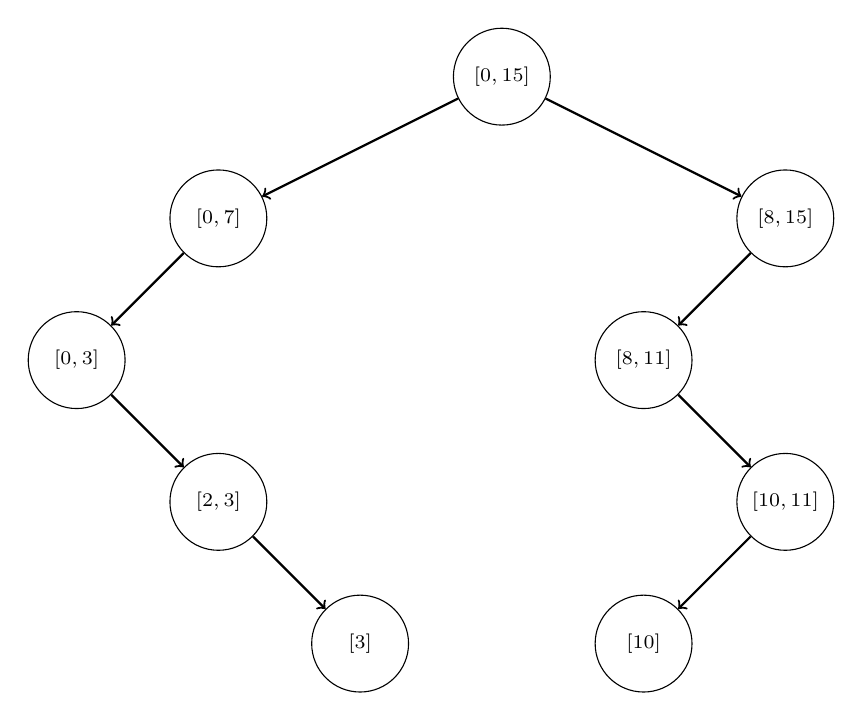
\begin{tikzpicture}[scale=0.9]
\scriptsize
\node[draw, circle,minimum size=35pt] (1) at (0,0) {$[0,15]$};
\node[draw, circle,minimum size=35pt] (2) at (-4,-2) {$[0,7]$};
\node[draw, circle,minimum size=35pt] (3) at (-6,-4) {$[0,3]$};
\node[draw, circle,minimum size=35pt] (4) at (-4,-6) {$[2,3]$};
\node[draw, circle,minimum size=35pt] (5) at (-2,-8) {$[3]$};
\node[draw, circle,minimum size=35pt] (6) at (4,-2) {$[8,15]$};
\node[draw, circle,minimum size=35pt] (7) at (2,-4) {$[8,11]$};
\node[draw, circle,minimum size=35pt] (8) at (4,-6) {$[10,11]$};
\node[draw, circle,minimum size=35pt] (9) at (2,-8) {$[10]$};

\path[draw,thick,->] (1) -- (2);
\path[draw,thick,->] (2) -- (3);
\path[draw,thick,->] (3) -- (4);
\path[draw,thick,->] (4) -- (5);

\path[draw,thick,->] (1) -- (6);
\path[draw,thick,->] (6) -- (7);
\path[draw,thick,->] (7) -- (8);
\path[draw,thick,->] (8) -- (9);
\end{tikzpicture}
\end{center}

Bất kỳ đường đi nào từ nút gốc đến một lá đều chứa
$O(\log n)$ nút,
vì vậy mỗi thao tác thêm nhiều nhất $O(\log n)$
nút mới vào cây.
Do đó, sau $k$ thao tác, cây chứa
nhiều nhất $O(k \log n)$ nút.

Lưu ý rằng nếu chúng ta biết tất cả các phần tử sẽ được cập nhật
khi bắt đầu thuật toán,
một cây phân đoạn động là không cần thiết,
bởi vì chúng ta có thể sử dụng một cây phân đoạn thông thường với
nén chỉ số (Chương 9.4).
Tuy nhiên, điều này là không thể khi các chỉ số
được tạo ra trong quá trình thuật toán.

\subsubsection{Cây phân đoạn bền bỉ}

\index{persistent segment tree}

Sử dụng một cách triển khai động,
cũng có thể tạo một
\key{cây phân đoạn bền bỉ (persistent segment tree)} lưu trữ
\emph{lịch sử sửa đổi} của cây.
Trong một cách triển khai như vậy, chúng ta có thể
truy cập hiệu quả
tất cả các phiên bản của cây đã
tồn tại trong quá trình thuật toán.

Khi lịch sử sửa đổi có sẵn,
chúng ta có thể thực hiện các truy vấn trong bất kỳ cây nào trước đó
giống như trong một cây phân đoạn thông thường, bởi vì
cấu trúc đầy đủ của mỗi cây được lưu trữ.
Chúng ta cũng có thể tạo các cây mới dựa trên các cây trước đó
và sửa đổi chúng một cách độc lập.

Hãy xem xét chuỗi cập nhật sau,
trong đó các nút màu đỏ thay đổi
và các nút khác vẫn giữ nguyên:

\begin{center}
\begin{tikzpicture}[scale=0.8]
\node[draw, circle,minimum size=13pt] (1a) at (3,0) {};
\node[draw, circle,minimum size=13pt] (2a) at (2,-1) {};
\node[draw, circle,minimum size=13pt] (3a) at (4,-1) {};
\node[draw, circle,minimum size=13pt] (4a) at (1.5,-2) {};
\node[draw, circle,minimum size=13pt] (5a) at (2.5,-2) {};
\node[draw, circle,minimum size=13pt] (6a) at (3.5,-2) {};
\node[draw, circle,minimum size=13pt] (7a) at (4.5,-2) {};
\path[draw,thick,->] (1a) -- (2a);
\path[draw,thick,->] (1a) -- (3a);
\path[draw,thick,->] (2a) -- (4a);
\path[draw,thick,->] (2a) -- (5a);
\path[draw,thick,->] (3a) -- (6a);
\path[draw,thick,->] (3a) -- (7a);

\node[draw, circle,minimum size=13pt,fill=red] (1b) at (3+5,0) {};
\node[draw, circle,minimum size=13pt,fill=red] (2b) at (2+5,-1) {};
\node[draw, circle,minimum size=13pt] (3b) at (4+5,-1) {};
\node[draw, circle,minimum size=13pt] (4b) at (1.5+5,-2) {};
\node[draw, circle,minimum size=13pt,fill=red] (5b) at (2.5+5,-2) {};
\node[draw, circle,minimum size=13pt] (6b) at (3.5+5,-2) {};
\node[draw, circle,minimum size=13pt] (7b) at (4.5+5,-2) {};
\path[draw,thick,->] (1b) -- (2b);
\path[draw,thick,->] (1b) -- (3b);
\path[draw,thick,->] (2b) -- (4b);
\path[draw,thick,->] (2b) -- (5b);
\path[draw,thick,->] (3b) -- (6b);
\path[draw,thick,->] (3b) -- (7b);

\node[draw, circle,minimum size=13pt,fill=red] (1c) at (3+10,0) {};
\node[draw, circle,minimum size=13pt] (2c) at (2+10,-1) {};
\node[draw, circle,minimum size=13pt,fill=red] (3c) at (4+10,-1) {};
\node[draw, circle,minimum size=13pt] (4c) at (1.5+10,-2) {};
\node[draw, circle,minimum size=13pt] (5c) at (2.5+10,-2) {};
\node[draw, circle,minimum size=13pt] (6c) at (3.5+10,-2) {};
\node[draw, circle,minimum size=13pt,fill=red] (7c) at (4.5+10,-2) {};
\path[draw,thick,->] (1c) -- (2c);
\path[draw,thick,->] (1c) -- (3c);
\path[draw,thick,->] (2c) -- (4c);
\path[draw,thick,->] (2c) -- (5c);
\path[draw,thick,->] (3c) -- (6c);
\path[draw,thick,->] (3c) -- (7c);

\node at (3,-3) {bước 1};
\node at (3+5,-3) {bước 2};
\node at (3+10,-3) {bước 3};
\end{tikzpicture}
\end{center}
Sau mỗi lần cập nhật, hầu hết các nút của cây
vẫn giữ nguyên,
vì vậy một cách hiệu quả để lưu trữ lịch sử sửa đổi
là biểu diễn mỗi cây trong lịch sử dưới dạng một sự kết hợp
của các nút mới và các cây con của các cây trước đó.
Trong ví dụ này, lịch sử sửa đổi có thể được
lưu trữ như sau:
\begin{center}
\begin{tikzpicture}[scale=0.8]
\path[use as bounding box] (0, 1) rectangle (16, -3.5);

\node[draw, circle,minimum size=13pt] (1a) at (3,0) {};
\node[draw, circle,minimum size=13pt] (2a) at (2,-1) {};
\node[draw, circle,minimum size=13pt] (3a) at (4,-1) {};
\node[draw, circle,minimum size=13pt] (4a) at (1.5,-2) {};
\node[draw, circle,minimum size=13pt] (5a) at (2.5,-2) {};
\node[draw, circle,minimum size=13pt] (6a) at (3.5,-2) {};
\node[draw, circle,minimum size=13pt] (7a) at (4.5,-2) {};
\path[draw,thick,->] (1a) -- (2a);
\path[draw,thick,->] (1a) -- (3a);
\path[draw,thick,->] (2a) -- (4a);
\path[draw,thick,->] (2a) -- (5a);
\path[draw,thick,->] (3a) -- (6a);
\path[draw,thick,->] (3a) -- (7a);

\node[draw, circle,minimum size=13pt,fill=red] (1b) at (3+5,0) {};
\node[draw, circle,minimum size=13pt,fill=red] (2b) at (2+5,-1) {};
\node[draw, circle,minimum size=13pt,fill=red] (5b) at (2.5+5,-2) {};
\path[draw,thick,->] (1b) -- (2b);

\draw[thick,->] (1b) .. controls (3+5+2,0-1) and (3+5,2.5) .. (3a);

\draw[thick,->] (2b) .. controls (2+5-0.5,-1-0.5) and (2,4.5) .. (4a);


\path[draw,thick,->] (2b) -- (5b);

\node[draw, circle,minimum size=13pt,fill=red] (1c) at (3+10,0) {};
\node[draw, circle,minimum size=13pt,fill=red] (3c) at (4+10,-1) {};
\node[draw, circle,minimum size=13pt,fill=red] (7c) at (4.5+10,-2) {};
\path[draw,thick,->] (1c) -- (2b);
\path[draw,thick,->] (1c) -- (3c);

\draw[thick,->] (3c) .. controls (2.5+5,-3) and (3.5,-3) .. (6a);

\path[draw,thick,->] (3c) -- (7c);

\node at (3,-3) {bước 1};
\node at (3+5,-3) {bước 2};
\node at (3+10,-3) {bước 3};
\end{tikzpicture}
\end{center}

Cấu trúc của mỗi cây trước đó có thể được
tái tạo bằng cách đi theo các con trỏ
bắt đầu từ nút gốc tương ứng.
Vì mỗi thao tác
chỉ thêm $O(\log n)$ nút mới vào cây,
có thể lưu trữ toàn bộ lịch sử sửa đổi của cây.

\section{Cấu trúc dữ liệu}

Thay vì các giá trị đơn lẻ, các nút trong một cây phân đoạn
cũng có thể chứa \emph{các cấu trúc dữ liệu} duy trì thông tin
về các phạm vi tương ứng.
Trong một cây như vậy, các thao tác mất
thời gian $O(f(n) \log n)$, trong đó $f(n)$ là
thời gian cần thiết để xử lý một nút duy nhất trong một thao tác.

Ví dụ, hãy xem xét một cây phân đoạn
hỗ trợ các truy vấn có dạng
"một phần tử $x$ xuất hiện bao nhiêu lần
trong phạm vi $[a,b]$?"
Ví dụ, phần tử 1 xuất hiện ba lần
trong phạm vi sau:

\begin{center}
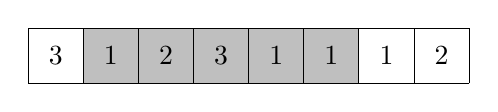
\begin{tikzpicture}[scale=0.7]
\fill[lightgray] (1,0) rectangle (6,1);
\draw (0,0) grid (8,1);

\node[anchor=center] at (0.5, 0.5) {3};
\node[anchor=center] at (1.5, 0.5) {1};
\node[anchor=center] at (2.5, 0.5) {2};
\node[anchor=center] at (3.5, 0.5) {3};
\node[anchor=center] at (4.5, 0.5) {1};
\node[anchor=center] at (5.5, 0.5) {1};
\node[anchor=center] at (6.5, 0.5) {1};
\node[anchor=center] at (7.5, 0.5) {2};
\end{tikzpicture}
\end{center}

Để hỗ trợ các truy vấn như vậy, chúng ta xây dựng một cây phân đoạn
trong đó mỗi nút được gán một cấu trúc dữ liệu
có thể được hỏi một phần tử $x$ bất kỳ xuất hiện bao nhiêu lần
trong phạm vi tương ứng.
Sử dụng cây này,
câu trả lời cho một truy vấn có thể được tính
bằng cách kết hợp các kết quả từ các nút
thuộc phạm vi.

Ví dụ, cây phân đoạn sau
tương ứng với mảng trên:
\begin{center}
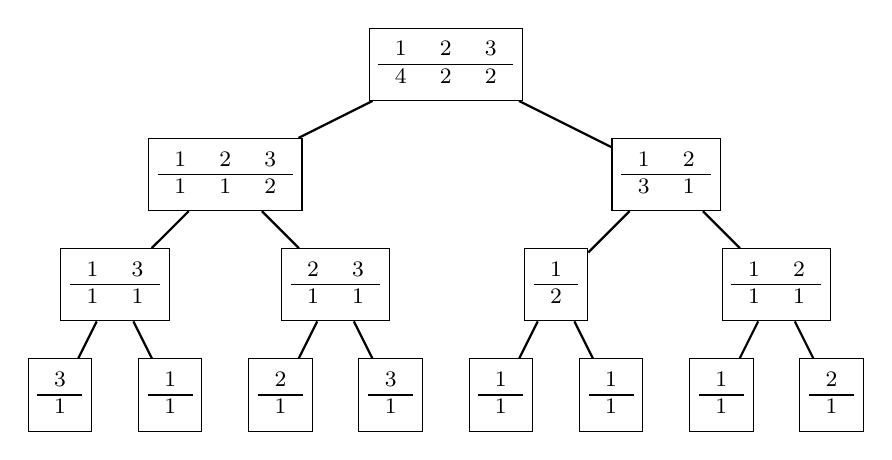
\begin{tikzpicture}[scale=0.7]

\node[draw, rectangle] (a) at (1,2.5)
{
\footnotesize
\begin{tabular}{r}
3 \\
\hline
1 \\
\end{tabular}};
\node[draw, rectangle] (b) at (3,2.5)
{
\footnotesize
\begin{tabular}{r}
1 \\
\hline
1 \\
\end{tabular}};
\node[draw, rectangle] (c) at (5,2.5)
{
\footnotesize
\begin{tabular}{r}
2 \\
\hline
1 \\
\end{tabular}};
\node[draw, rectangle] (d) at (7,2.5)
{
\footnotesize
\begin{tabular}{r}
3 \\
\hline
1 \\
\end{tabular}};
\node[draw, rectangle] (e) at (9,2.5)
{
\footnotesize
\begin{tabular}{r}
1 \\
\hline
1 \\
\end{tabular}};
\node[draw, rectangle] (f) at (11,2.5)
{
\footnotesize
\begin{tabular}{r}
1 \\
\hline
1 \\
\end{tabular}};
\node[draw, rectangle] (g) at (13,2.5)
{
\footnotesize
\begin{tabular}{r}
1 \\
\hline
1 \\
\end{tabular}};
\node[draw, rectangle] (h) at (15,2.5)
{
\footnotesize
\begin{tabular}{r}
2 \\
\hline
1 \\
\end{tabular}};

\node[draw, rectangle] (i) at (2,4.5)
{
\footnotesize
\begin{tabular}{rr}
1 & 3 \\
\hline
1 & 1 \\
\end{tabular}};
\path[draw,thick,-] (i) -- (a);
\path[draw,thick,-] (i) -- (b);
\node[draw, rectangle] (j) at (6,4.5)
{
\footnotesize
\begin{tabular}{rr}
2 & 3 \\
\hline
1 & 1 \\
\end{tabular}};
\path[draw,thick,-] (j) -- (c);
\path[draw,thick,-] (j) -- (d);
\node[draw, rectangle] (k) at (10,4.5)
{
\footnotesize
\begin{tabular}{r}
1 \\
\hline
2 \\
\end{tabular}};
\path[draw,thick,-] (k) -- (e);
\path[draw,thick,-] (k) -- (f);
\node[draw, rectangle] (l) at (14,4.5)
{
\footnotesize
\begin{tabular}{rr}
1 & 2 \\
\hline
1 & 1 \\
\end{tabular}};
\path[draw,thick,-] (l) -- (g);
\path[draw,thick,-] (l) -- (h);

\node[draw, rectangle] (m) at (4,6.5)
{
\footnotesize
\begin{tabular}{rrr}
1 & 2 & 3 \\
\hline
1 & 1 & 2 \\
\end{tabular}};
\path[draw,thick,-] (m) -- (i);
\path[draw,thick,-] (m) -- (j);
\node[draw, rectangle] (n) at (12,6.5)
{
\footnotesize
\begin{tabular}{rr}
1 & 2 \\
\hline
3 & 1 \\
\end{tabular}};
\path[draw,thick,-] (n) -- (k);
\path[draw,thick,-] (n) -- (l);

\node[draw, rectangle] (o) at (8,8.5)
{
\footnotesize
\begin{tabular}{rrr}
1 & 2 & 3 \\
\hline
4 & 2 & 2 \\
\end{tabular}};
\path[draw,thick,-] (o) -- (m);
\path[draw,thick,-] (o) -- (n);
\end{tikzpicture}
\end{center}

Chúng ta có thể xây dựng cây sao cho
mỗi nút chứa một cấu trúc \texttt{map}.
Trong trường hợp này, thời gian cần thiết để xử lý mỗi
nút là $O(\log n)$, vì vậy tổng độ phức tạp thời gian
của một truy vấn là $O(\log^2 n)$.
Cây sử dụng $O(n \log n)$ bộ nhớ,
bởi vì có $O(\log n)$ cấp
và mỗi cấp chứa
$O(n)$ phần tử.

\section{Hai chiều}

\index{two-dimensional segment tree}

Một \key{cây phân đoạn hai chiều (two-dimensional segment tree)} hỗ trợ
các truy vấn liên quan đến các mảng con hình chữ nhật
của một mảng hai chiều.
Một cây như vậy có thể được triển khai dưới dạng
các cây phân đoạn lồng nhau: một cây lớn tương ứng với
các hàng của mảng, và mỗi nút chứa một cây nhỏ
tương ứng với một cột.

Ví dụ, trong mảng
\begin{center}
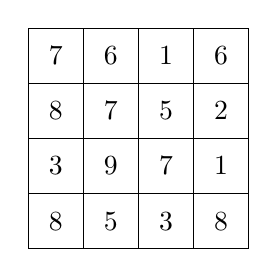
\begin{tikzpicture}[scale=0.7]
\draw (0,0) grid (4,4);

\node[anchor=center] at (0.5, 0.5) {8};
\node[anchor=center] at (1.5, 0.5) {5};
\node[anchor=center] at (2.5, 0.5) {3};
\node[anchor=center] at (3.5, 0.5) {8};

\node[anchor=center] at (0.5, 1.5) {3};
\node[anchor=center] at (1.5, 1.5) {9};
\node[anchor=center] at (2.5, 1.5) {7};
\node[anchor=center] at (3.5, 1.5) {1};

\node[anchor=center] at (0.5, 2.5) {8};
\node[anchor=center] at (1.5, 2.5) {7};
\node[anchor=center] at (2.5, 2.5) {5};
\node[anchor=center] at (3.5, 2.5) {2};

\node[anchor=center] at (0.5, 3.5) {7};
\node[anchor=center] at (1.5, 3.5) {6};
\node[anchor=center] at (2.5, 3.5) {1};
\node[anchor=center] at (3.5, 3.5) {6};
\end{tikzpicture}
\end{center}
tổng của bất kỳ mảng con nào
cũng có thể được tính
từ cây phân đoạn sau:
\begin{center}
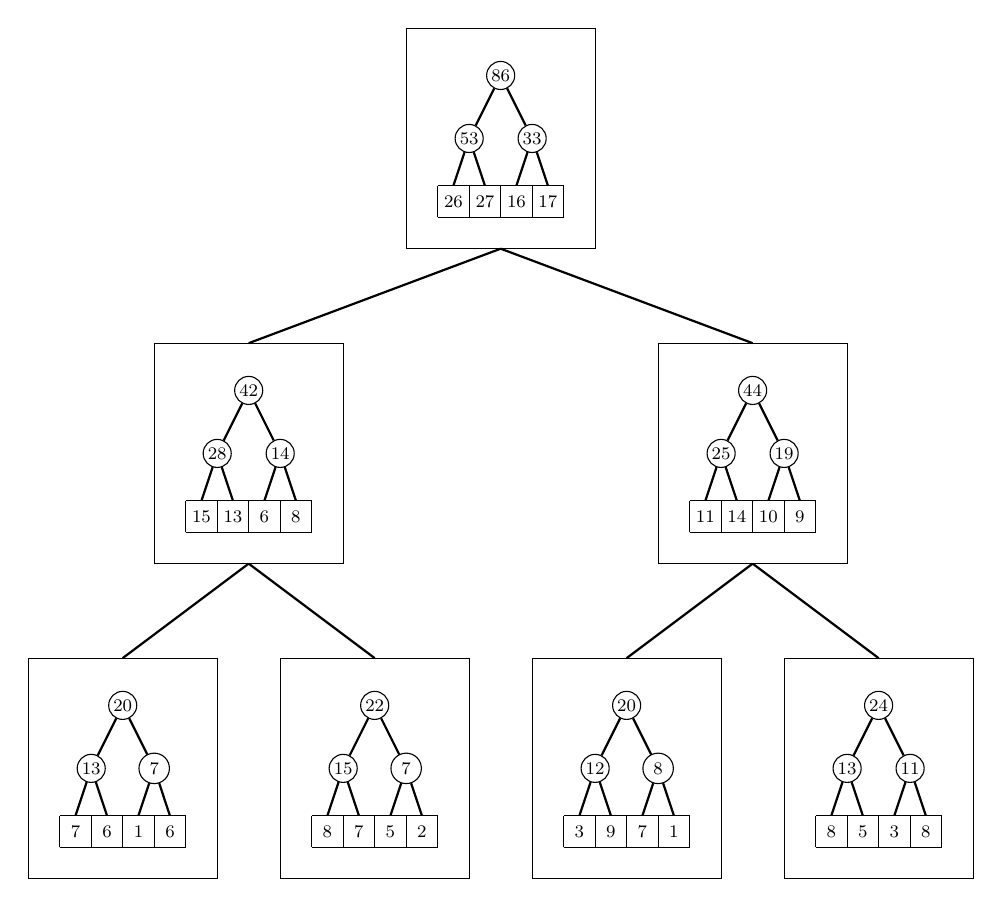
\begin{tikzpicture}[scale=0.4]
\footnotesize
\begin{scope}[shift={(-12,0)}]
\draw (-1,-1) rectangle (5,6);
\draw (0,0) grid (4,1);
\node[anchor=center,scale=0.8] at (0.5, 0.5) {7};
\node[anchor=center,scale=0.8] at (1.5, 0.5) {6};
\node[anchor=center,scale=0.8] at (2.5, 0.5) {1};
\node[anchor=center,scale=0.8] at (3.5, 0.5) {6};

\node[draw, circle,scale=0.8,inner sep=1pt] (a) at (1,2.5) {13};
\path[draw,thick,-] (a) -- (0.5,1);
\path[draw,thick,-] (a) -- (1.5,1);
\node[draw, circle,scale=0.8,inner sep=2.5pt] (b) at (3,2.5) {7};
\path[draw,thick,-] (b) -- (2.5,1);
\path[draw,thick,-] (b) -- (3.5,1);

\node[draw, circle,scale=0.8,inner sep=1pt] (i) at (2,4.5) {20};
\path[draw,thick,-] (i) -- (a);
\path[draw,thick,-] (i) -- (b);
\end{scope}
\begin{scope}[shift={(-4,0)}]
\draw (-1,-1) rectangle (5,6);
\draw (0,0) grid (4,1);
\node[anchor=center,scale=0.8] at (0.5, 0.5) {8};
\node[anchor=center,scale=0.8] at (1.5, 0.5) {7};
\node[anchor=center,scale=0.8] at (2.5, 0.5) {5};
\node[anchor=center,scale=0.8] at (3.5, 0.5) {2};

\node[draw, circle,scale=0.8,inner sep=1pt] (a) at (1,2.5) {15};
\path[draw,thick,-] (a) -- (0.5,1);
\path[draw,thick,-] (a) -- (1.5,1);
\node[draw, circle,scale=0.8,inner sep=2.5pt] (b) at (3,2.5) {7};
\path[draw,thick,-] (b) -- (2.5,1);
\path[draw,thick,-] (b) -- (3.5,1);

\node[draw, circle,scale=0.8,inner sep=1pt] (i) at (2,4.5) {22};
\path[draw,thick,-] (i) -- (a);
\path[draw,thick,-] (i) -- (b);
\end{scope}
\begin{scope}[shift={(4,0)}]
\draw (-1,-1) rectangle (5,6);
\draw (0,0) grid (4,1);
\node[anchor=center,scale=0.8] at (0.5, 0.5) {3};
\node[anchor=center,scale=0.8] at (1.5, 0.5) {9};
\node[anchor=center,scale=0.8] at (2.5, 0.5) {7};
\node[anchor=center,scale=0.8] at (3.5, 0.5) {1};

\node[draw, circle,scale=0.8,inner sep=1pt] (a) at (1,2.5) {12};
\path[draw,thick,-] (a) -- (0.5,1);
\path[draw,thick,-] (a) -- (1.5,1);
\node[draw, circle,scale=0.8,inner sep=2.5pt] (b) at (3,2.5) {8};
\path[draw,thick,-] (b) -- (2.5,1);
\path[draw,thick,-] (b) -- (3.5,1);

\node[draw, circle,scale=0.8,inner sep=1pt] (i) at (2,4.5) {20};
\path[draw,thick,-] (i) -- (a);
\path[draw,thick,-] (i) -- (b);
\end{scope}
\begin{scope}[shift={(12,0)}]
\draw (-1,-1) rectangle (5,6);
\draw (0,0) grid (4,1);
\node[anchor=center,scale=0.8] at (0.5, 0.5) {8};
\node[anchor=center,scale=0.8] at (1.5, 0.5) {5};
\node[anchor=center,scale=0.8] at (2.5, 0.5) {3};
\node[anchor=center,scale=0.8] at (3.5, 0.5) {8};

\node[draw, circle,scale=0.8,inner sep=1pt] (a) at (1,2.5) {13};
\path[draw,thick,-] (a) -- (0.5,1);
\path[draw,thick,-] (a) -- (1.5,1);
\node[draw, circle,scale=0.8,inner sep=1pt] (b) at (3,2.5) {11};
\path[draw,thick,-] (b) -- (2.5,1);
\path[draw,thick,-] (b) -- (3.5,1);

\node[draw, circle,scale=0.8,inner sep=1pt] (i) at (2,4.5) {24};
\path[draw,thick,-] (i) -- (a);
\path[draw,thick,-] (i) -- (b);
\end{scope}
\begin{scope}[shift={(-8,10)}]
\draw (-1,-1) rectangle (5,6);
\draw (0,0) grid (4,1);
\node[anchor=center,scale=0.8] at (0.5, 0.5) {15};
\node[anchor=center,scale=0.8] at (1.5, 0.5) {13};
\node[anchor=center,scale=0.8] at (2.5, 0.5) {6};
\node[anchor=center,scale=0.8] at (3.5, 0.5) {8};

\node[draw, circle,scale=0.8,inner sep=1pt] (a) at (1,2.5) {28};
\path[draw,thick,-] (a) -- (0.5,1);
\path[draw,thick,-] (a) -- (1.5,1);
\node[draw, circle,scale=0.8,inner sep=1pt] (b) at (3,2.5) {14};
\path[draw,thick,-] (b) -- (2.5,1);
\path[draw,thick,-] (b) -- (3.5,1);

\node[draw, circle,scale=0.8,inner sep=1pt] (i) at (2,4.5) {42};
\path[draw,thick,-] (i) -- (a);
\path[draw,thick,-] (i) -- (b);
\end{scope}
\begin{scope}[shift={(8,10)}]
\draw (-1,-1) rectangle (5,6);
\draw (0,0) grid (4,1);
\node[anchor=center,scale=0.8] at (0.5, 0.5) {11};
\node[anchor=center,scale=0.8] at (1.5, 0.5) {14};
\node[anchor=center,scale=0.8] at (2.5, 0.5) {10};
\node[anchor=center,scale=0.8] at (3.5, 0.5) {9};

\node[draw, circle,scale=0.8,inner sep=1pt] (a) at (1,2.5) {25};
\path[draw,thick,-] (a) -- (0.5,1);
\path[draw,thick,-] (a) -- (1.5,1);
\node[draw, circle,scale=0.8,inner sep=1pt] (b) at (3,2.5) {19};
\path[draw,thick,-] (b) -- (2.5,1);
\path[draw,thick,-] (b) -- (3.5,1);

\node[draw, circle,scale=0.8,inner sep=1pt] (i) at (2,4.5) {44};
\path[draw,thick,-] (i) -- (a);
\path[draw,thick,-] (i) -- (b);
\end{scope}
\begin{scope}[shift={(0,20)}]
\draw (-1,-1) rectangle (5,6);
\draw (0,0) grid (4,1);
\node[anchor=center,scale=0.8] at (0.5, 0.5) {26};
\node[anchor=center,scale=0.8] at (1.5, 0.5) {27};
\node[anchor=center,scale=0.8] at (2.5, 0.5) {16};
\node[anchor=center,scale=0.8] at (3.5, 0.5) {17};

\node[draw, circle,scale=0.8,inner sep=1pt] (a) at (1,2.5) {53};
\path[draw,thick,-] (a) -- (0.5,1);
\path[draw,thick,-] (a) -- (1.5,1);
\node[draw, circle,scale=0.8,inner sep=1pt] (b) at (3,2.5) {33};
\path[draw,thick,-] (b) -- (2.5,1);
\path[draw,thick,-] (b) -- (3.5,1);

\node[draw, circle,scale=0.8,inner sep=1pt] (i) at (2,4.5) {86};
\path[draw,thick,-] (i) -- (a);
\path[draw,thick,-] (i) -- (b);
\end{scope}
\path[draw,thick,-] (2,19) -- (-6,16);
\path[draw,thick,-] (2,19) -- (10,16);
\path[draw,thick,-] (-6,9) -- (-10,6);
\path[draw,thick,-] (-6,9) -- (-2,6);
\path[draw,thick,-] (10,9) -- (6,6);
\path[draw,thick,-] (10,9) -- (14,6);
\end{tikzpicture}
\end{center}

Các thao tác của một cây phân đoạn hai chiều
mất thời gian $O(\log^2 n)$, bởi vì cây lớn
và mỗi cây nhỏ bao gồm $O(\log n)$ cấp.
Cây yêu cầu $O(n^2)$ bộ nhớ, bởi vì mỗi
cây nhỏ chứa $O(n)$ giá trị.